\documentclass[12pt]{beamer}
\setbeamertemplate{navigation symbols}{}
%\usepackage[latin1]{inputenc}
\usepackage{pgfplots}
\usepackage{adjustbox}
\usepackage{graphicx}
%\usepackage{draftwatermark}
\usepackage{tikz}
\usepackage{colortbl}
\usepackage{subfigure}
%\usetheme{Amsterdam}
\usecolortheme{default}
\title[]{Government websites as data: A methodological pipeline for
collection, processing, and text analysis}
\author{Markus Neumann \\ Fridolin Linder \\ Bruce Desmarais}
\institute{The Pennsylvania State University}
\date{January 6, 2018}

\makeatletter
\defbeamertemplate*{footline}{myminiframes theme}
{%
	\begin{beamercolorbox}[colsep=1.5pt]{upper separation line foot}
	\end{beamercolorbox}
	\hbox{%
		\begin{beamercolorbox}[wd=.1\paperwidth,ht=2.5ex,dp=1.125ex,%
			leftskip=.3cm,rightskip=.3cm,center]{title in head/foot}%
			{\usebeamerfont{author in head/foot}\usebeamercolor[fg]{author in head/foot}}{\insertframenumber}%/\inserttotalframenumber}%
		\end{beamercolorbox}%
		\begin{beamercolorbox}[wd=.75\paperwidth,ht=2.5ex,dp=1.125ex,%
			leftskip=.3cm,rightskip=.3cm plus1fil,center]{title in head/foot}%
			\leavevmode{\usebeamerfont{title in head/foot}\insertshorttitle}%
		\end{beamercolorbox}%
		\begin{beamercolorbox}[wd=.15\paperwidth,ht=2.5ex,dp=1.125ex,%
			leftskip=.3cm,rightskip=.3cm plus1fil,center]{title in head/foot}%
			{\usebeamerfont{author in head/foot}\usebeamercolor[fg]{author in head/foot}}%\insertshortauthor}
		\end{beamercolorbox}%
	}%
	\begin{beamercolorbox}[colsep=1.5pt]{lower separation line foot}
	\end{beamercolorbox}
}
\makeatother

\begin{document}

\section{Introduction}
\begin{frame}
\titlepage
\end{frame}

%\begin{frame}{Spot the difference}
%\begin{figure}
%	\hfill
%	\subfigure{\includegraphics[width=5cm]{Images/Clinton_Rally_cr.jpg}}
%	\hfill
%	\subfigure{\includegraphics[width=5cm]{Images/Trump_Rally_cr.jpg}}
%\end{figure}
%\end{frame}

\begin{frame}{Government Websites}
\linespread{1.5}
{\large
	\begin{itemize}
		\item Content of government websites is an important source of information \& transparency
		\item After coming into power, the Trump administration  has made some controversial changes to the websites of federal agencies
		\item Website content is political
		\item Partisanship of city government is expected to have an effect
	\end{itemize}
	
}
\end{frame}

\begin{frame}{Example Website}
	
\includegraphics[width = \linewidth]{arcadia_water.png}
\end{frame}

\begin{frame}{Local Government Websites}
\linespread{1.5}
{\large
	\begin{itemize}
		\item Most local (i.e. mayoral) elections are non-partisan
		\item Few states have exclusively partisan local elections
		\item Data for these elections can be difficult to find
		\item We selected Indiana and Louisiana
	\end{itemize}
	
	}
\end{frame}

\begin{frame}{Data Overview}
\begin{figure}
	\hfill
	\subfigure{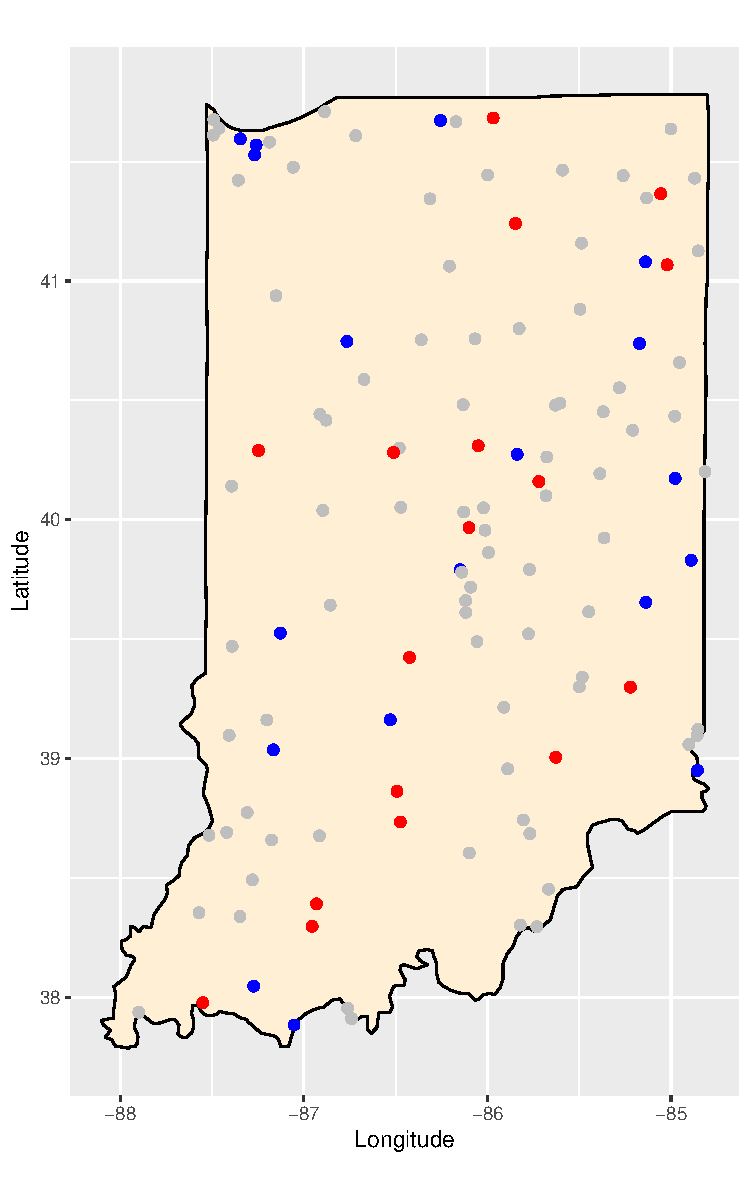
\includegraphics[width=5cm, height = .7\textheight]{../figures/indiana_map.pdf}}
	\hfill
	\subfigure{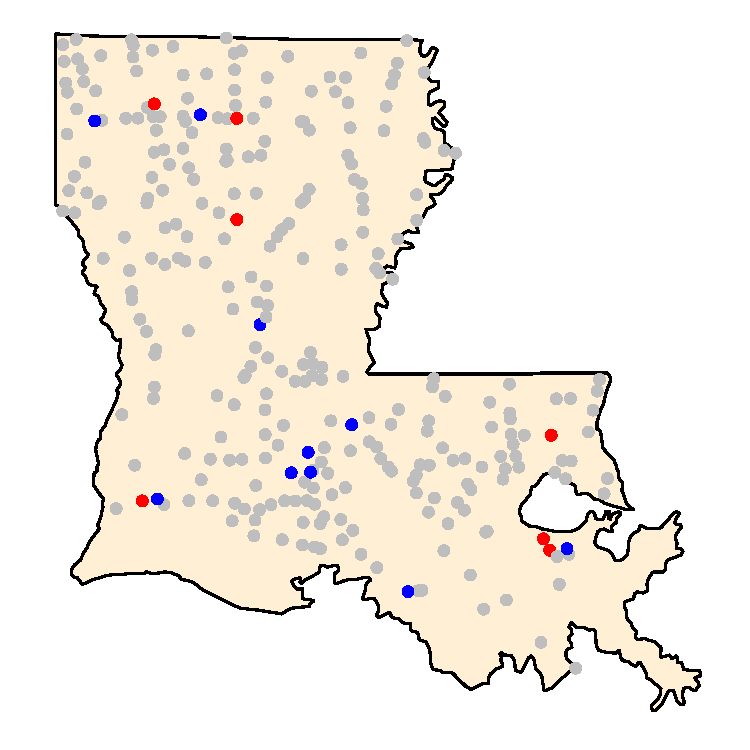
\includegraphics[width=5cm, height = .7\textheight]{../figures/louisiana_map.pdf}}
\end{figure}
\end{frame}

\begin{frame}{Literature}
\linespread{1.5}
{\large
	\begin{itemize}
		\item Extant literature largely focuses on e-government and transparency, for example:
		\begin{itemize}
			\item Wang, Bretschneider and Gant (2005)
			\item Grimmelikhuijsen \& Welch (2012)
			\item Dolson \& Young (2012)
			\item Feeney \& Brown (2017)
		\end{itemize}
		\item All of these papers rely on manual website coding
	\end{itemize}
	
}
\end{frame}

\begin{frame}{The Pipeline}
	\textbf{Data Collection} \hspace{2mm} $\rightarrow$ \hspace{2mm} \textbf{Preprocessing} \hspace{2mm} $\rightarrow$ \hspace{2mm} \textbf{Analysis}
\begin{columns}
	\column{0.33\textwidth}
	%Data Collection
	\vspace{5mm}
	\begin{itemize}
		\item Identify URLs
		\item Verify URLs (browser automation)
		\item Download websites
		\item Determine file type
		\item Convert to txt
	\end{itemize}		
	\column{0.33\textwidth}
	%Preprocessing
	\vspace{5mm}
	\begin{itemize}
		\item Remove punctuation, dates, etc.
		\item To lowercase
		\item Boilerplate removal
		\item Spellchecking
		\item Lemmatization \\ (city \& cities = city)
	\end{itemize}
	\column{0.33\textwidth}
	%Analysis
	\vspace{5mm}
	\begin{itemize}
		%\item Hierarchical clustering
		\item Fightin' Words
		\item Structural topic model
		%\begin{itemize}
		%	\item LDA
		%	\item STM
		%\end{itemize}
	\end{itemize}
\end{columns}
\end{frame}

\begin{frame}{The Pipeline}
	\textbf{Data Collection} \hspace{2mm} $\rightarrow$ \hspace{2mm} \textbf{Preprocessing} \hspace{2mm} $\rightarrow$ \hspace{2mm} \textbf{Analysis}
	\begin{columns}
		\column{0.33\textwidth}
		%Data Collection
		\vspace{5mm}
		\begin{itemize}
			\item Identify URLs
			\item Verify URLs (browser automation)
			\item Download websites
			\item Determine file type
			\item Convert to txt
		\end{itemize}		
		\column{0.33\textwidth}
		%Preprocessing
		\vspace{5mm}
		\begin{itemize}
			\item Remove punctuation, dates, etc.
			\item To lowercase
			\item \textbf{Boilerplate removal}
			\item Spellchecking
			\item Lemmatization \\ (city \& cities = city)
		\end{itemize}
		\column{0.33\textwidth}
		%Analysis
		\vspace{5mm}
		\begin{itemize}
			%\item Hierarchical clustering
			\item Fightin' Words
			\item Structural topic model
			%\begin{itemize}
			%	\item LDA
			%	\item STM
			%\end{itemize}
		\end{itemize}
	\end{columns}
\end{frame}

\section{Preprocessing}

%\begin{frame}{Document filetype \& conversion}
%\begin{itemize}
%	\item Websites contain a number of different filetypes
%	\item txt, pdf, html, doc and docx are useable
%	\item convert everything to txt
%	\item the file ENDING does not always 
%\end{itemize}
%\end{frame}

\begin{frame}{Boilerplate Removal}

\includegraphics[width = \linewidth]{arcadia_water.png}
\end{frame}

\begin{frame}{Boilerplate Removal}
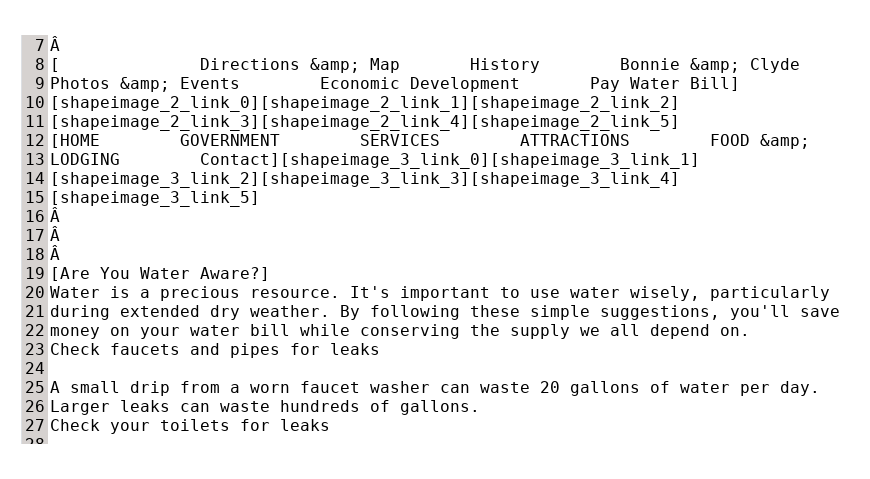
\includegraphics[width = \linewidth]{duplicateLines.png}
\end{frame}

\begin{frame}{Boilerplate Removal}
	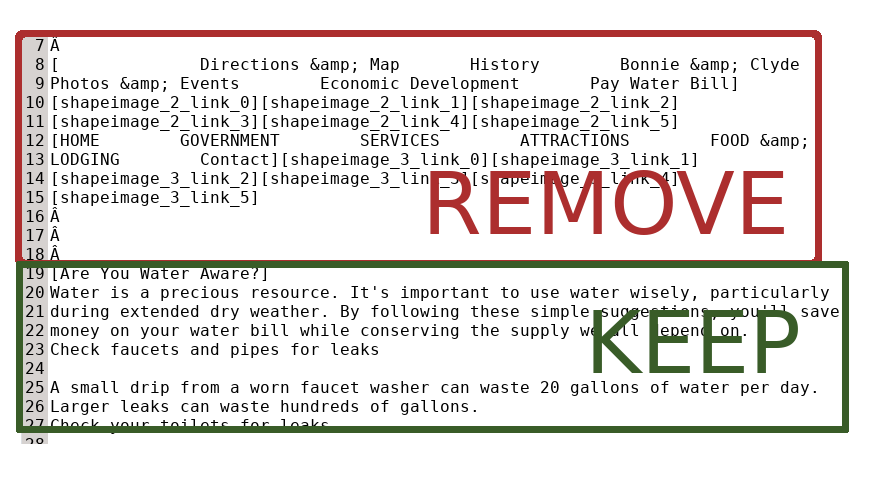
\includegraphics[width = \linewidth]{duplicateLineRemoval.png}
\end{frame}

\begin{frame}{Boilerplate Removal}
\begin{itemize}
	\item Within each city, there is a lot of shared text
	\item If not removed, the text clusters into cities
\end{itemize}
\begin{itemize}
	\item Solution: Compare each line in each document to every other line in every document of that city
	\item Count duplicates
	\item Remove a line if it is duplicated within a city above some threshold
	\item Fast \& efficient implementation
\end{itemize}
\end{frame}

\begin{frame}{The Pipeline}
	\textbf{Data Collection} \hspace{2mm} $\rightarrow$ \hspace{2mm} \textbf{Preprocessing} \hspace{2mm} $\rightarrow$ \hspace{2mm} \textbf{Analysis}
	\begin{columns}
		\column{0.33\textwidth}
		%Data Collection
		\vspace{5mm}
		\begin{itemize}
			\item Identify URLs
			\item Verify URLs (browser automation)
			\item Download websites
			\item Determine file type
			\item Convert to txt
		\end{itemize}		
		\column{0.33\textwidth}
		%Preprocessing
		\vspace{5mm}
		\begin{itemize}
			\item Remove punctuation, dates, etc.
			\item To lowercase
			\item Boilerplate removal
			\item Spellchecking
			\item Lemmatization \\ (city \& cities = city)
		\end{itemize}
		\column{0.33\textwidth}
		%Analysis
		\vspace{5mm}
		\begin{itemize}
			%\item Hierarchical clustering
			\item Fightin' Words
			\item Structural topic model
			%\begin{itemize}
			%	\item LDA
			%	\item STM
			%\end{itemize}
		\end{itemize}
	\end{columns}
\end{frame}

%\begin{frame}{Other preprocessing}
%\begin{itemize}
%	\item Remove:
%	\begin{itemize}
%		\item Dates
%		\item Numbers
%		\item Punctuation
%		\item Words not recognized by an English dictionary
%		\item Stopwords
%		\item Documents with too few unique words
%	\end{itemize}
%\item Set to lowercase
%\item Lemmatization
%\end{itemize}
%\end{frame}

\begin{frame}{Data Overview}
% latex table generated in R 3.4.2 by xtable 1.8-2 package
% Wed Dec 27 19:51:57 2017
\begin{table}[ht]
\centering
\begin{tabular}{rrrr}
  \hline
 & Democratic & Republican & Total \\ 
  \hline
Cities & 16 & 17 & 33 \\ 
  Documents & 10868 & 6438 & 17306 \\ 
  Token types & 20774 & 17947 & 21697 \\ 
  Token instances & 6532383 & 2651876 & 9184259 \\ 
   \hline
\end{tabular}
\caption{Indiana} 
\end{table}


% latex table generated in R 3.4.2 by xtable 1.8-2 package
% Wed Dec 27 19:55:34 2017
\begin{table}[ht]
\centering
\begin{tabular}{rrrr}
  \hline
 & Democratic & Republican & Total \\ 
  \hline
Cities & 10 & 8 & 18 \\ 
  Documents & 6636 & 1378 & 8014 \\ 
  Token types & 16649 & 9234 & 16856 \\ 
  Token instances & 3764877 & 355774 & 4120651 \\ 
   \hline
\end{tabular}
\caption{Louisiana} 
\end{table}


\end{frame}

\section{Analysis}
%\begin{frame}{Hierarchical Clustering}
%\centering
%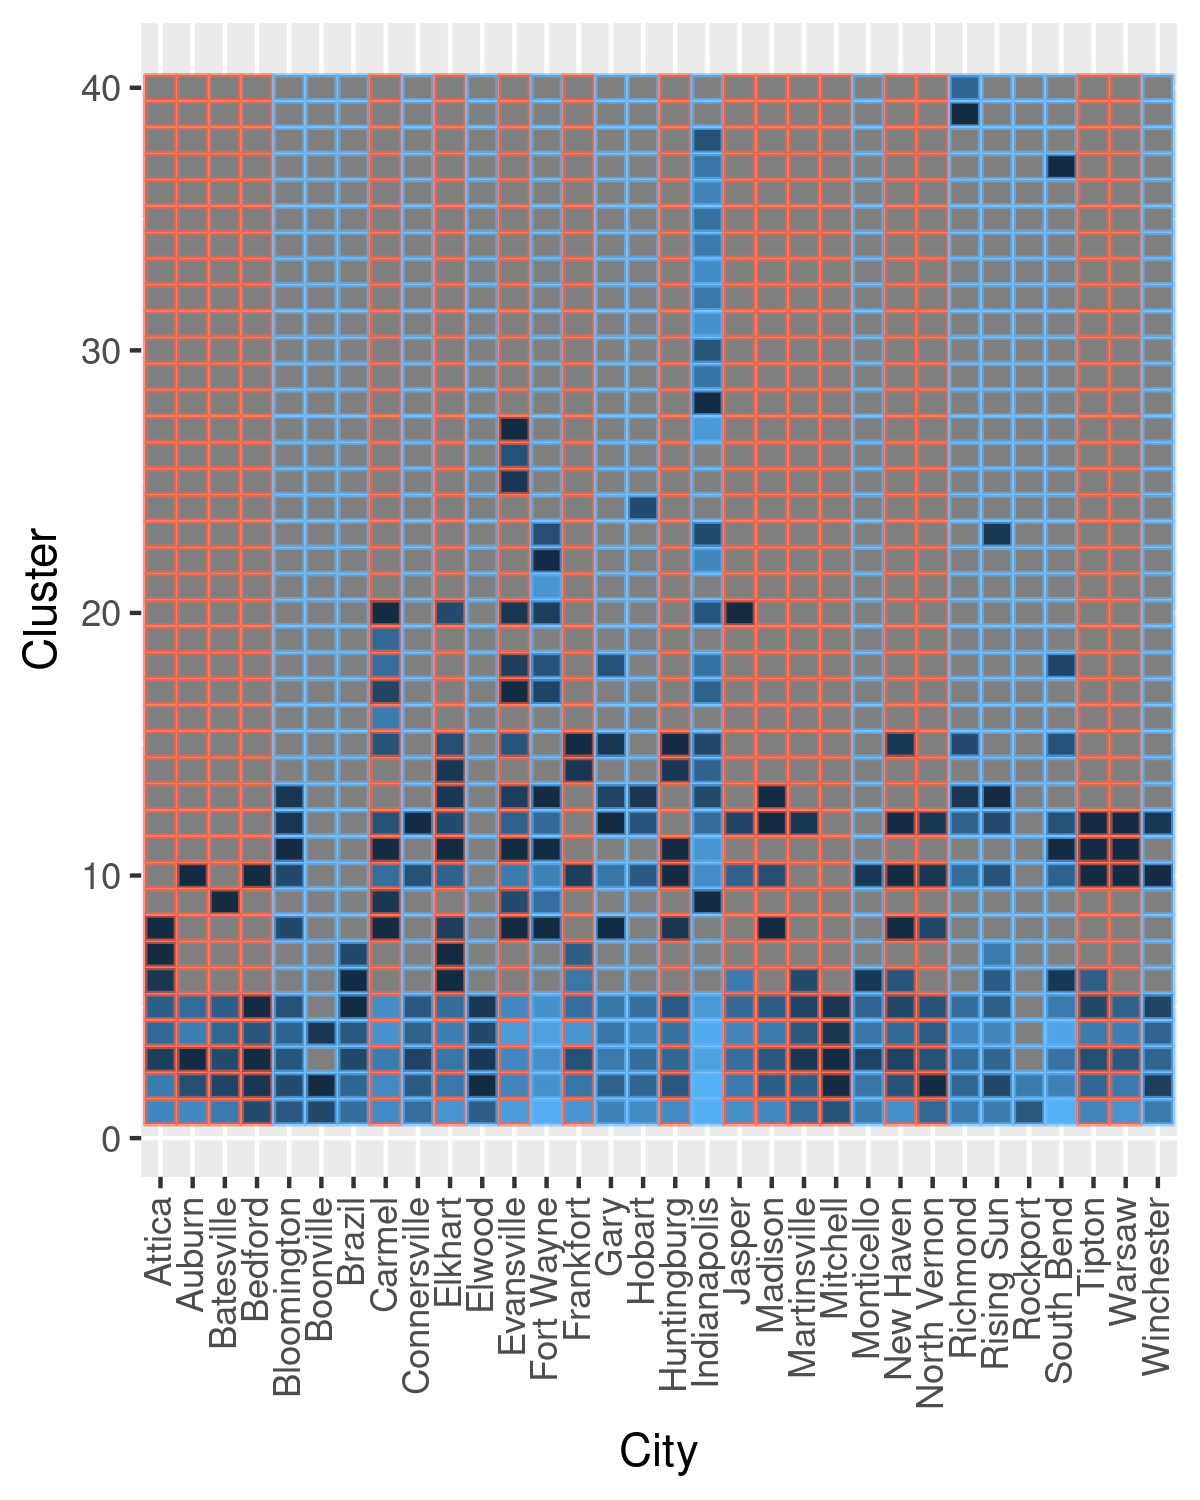
\includegraphics[height=\textheight]{../figures/heatmap_hclust_40.png}
%\end{frame}

%\begin{frame}{Fightin' Words}
%\begin{figure}
%	\hfill
%	\subfigure{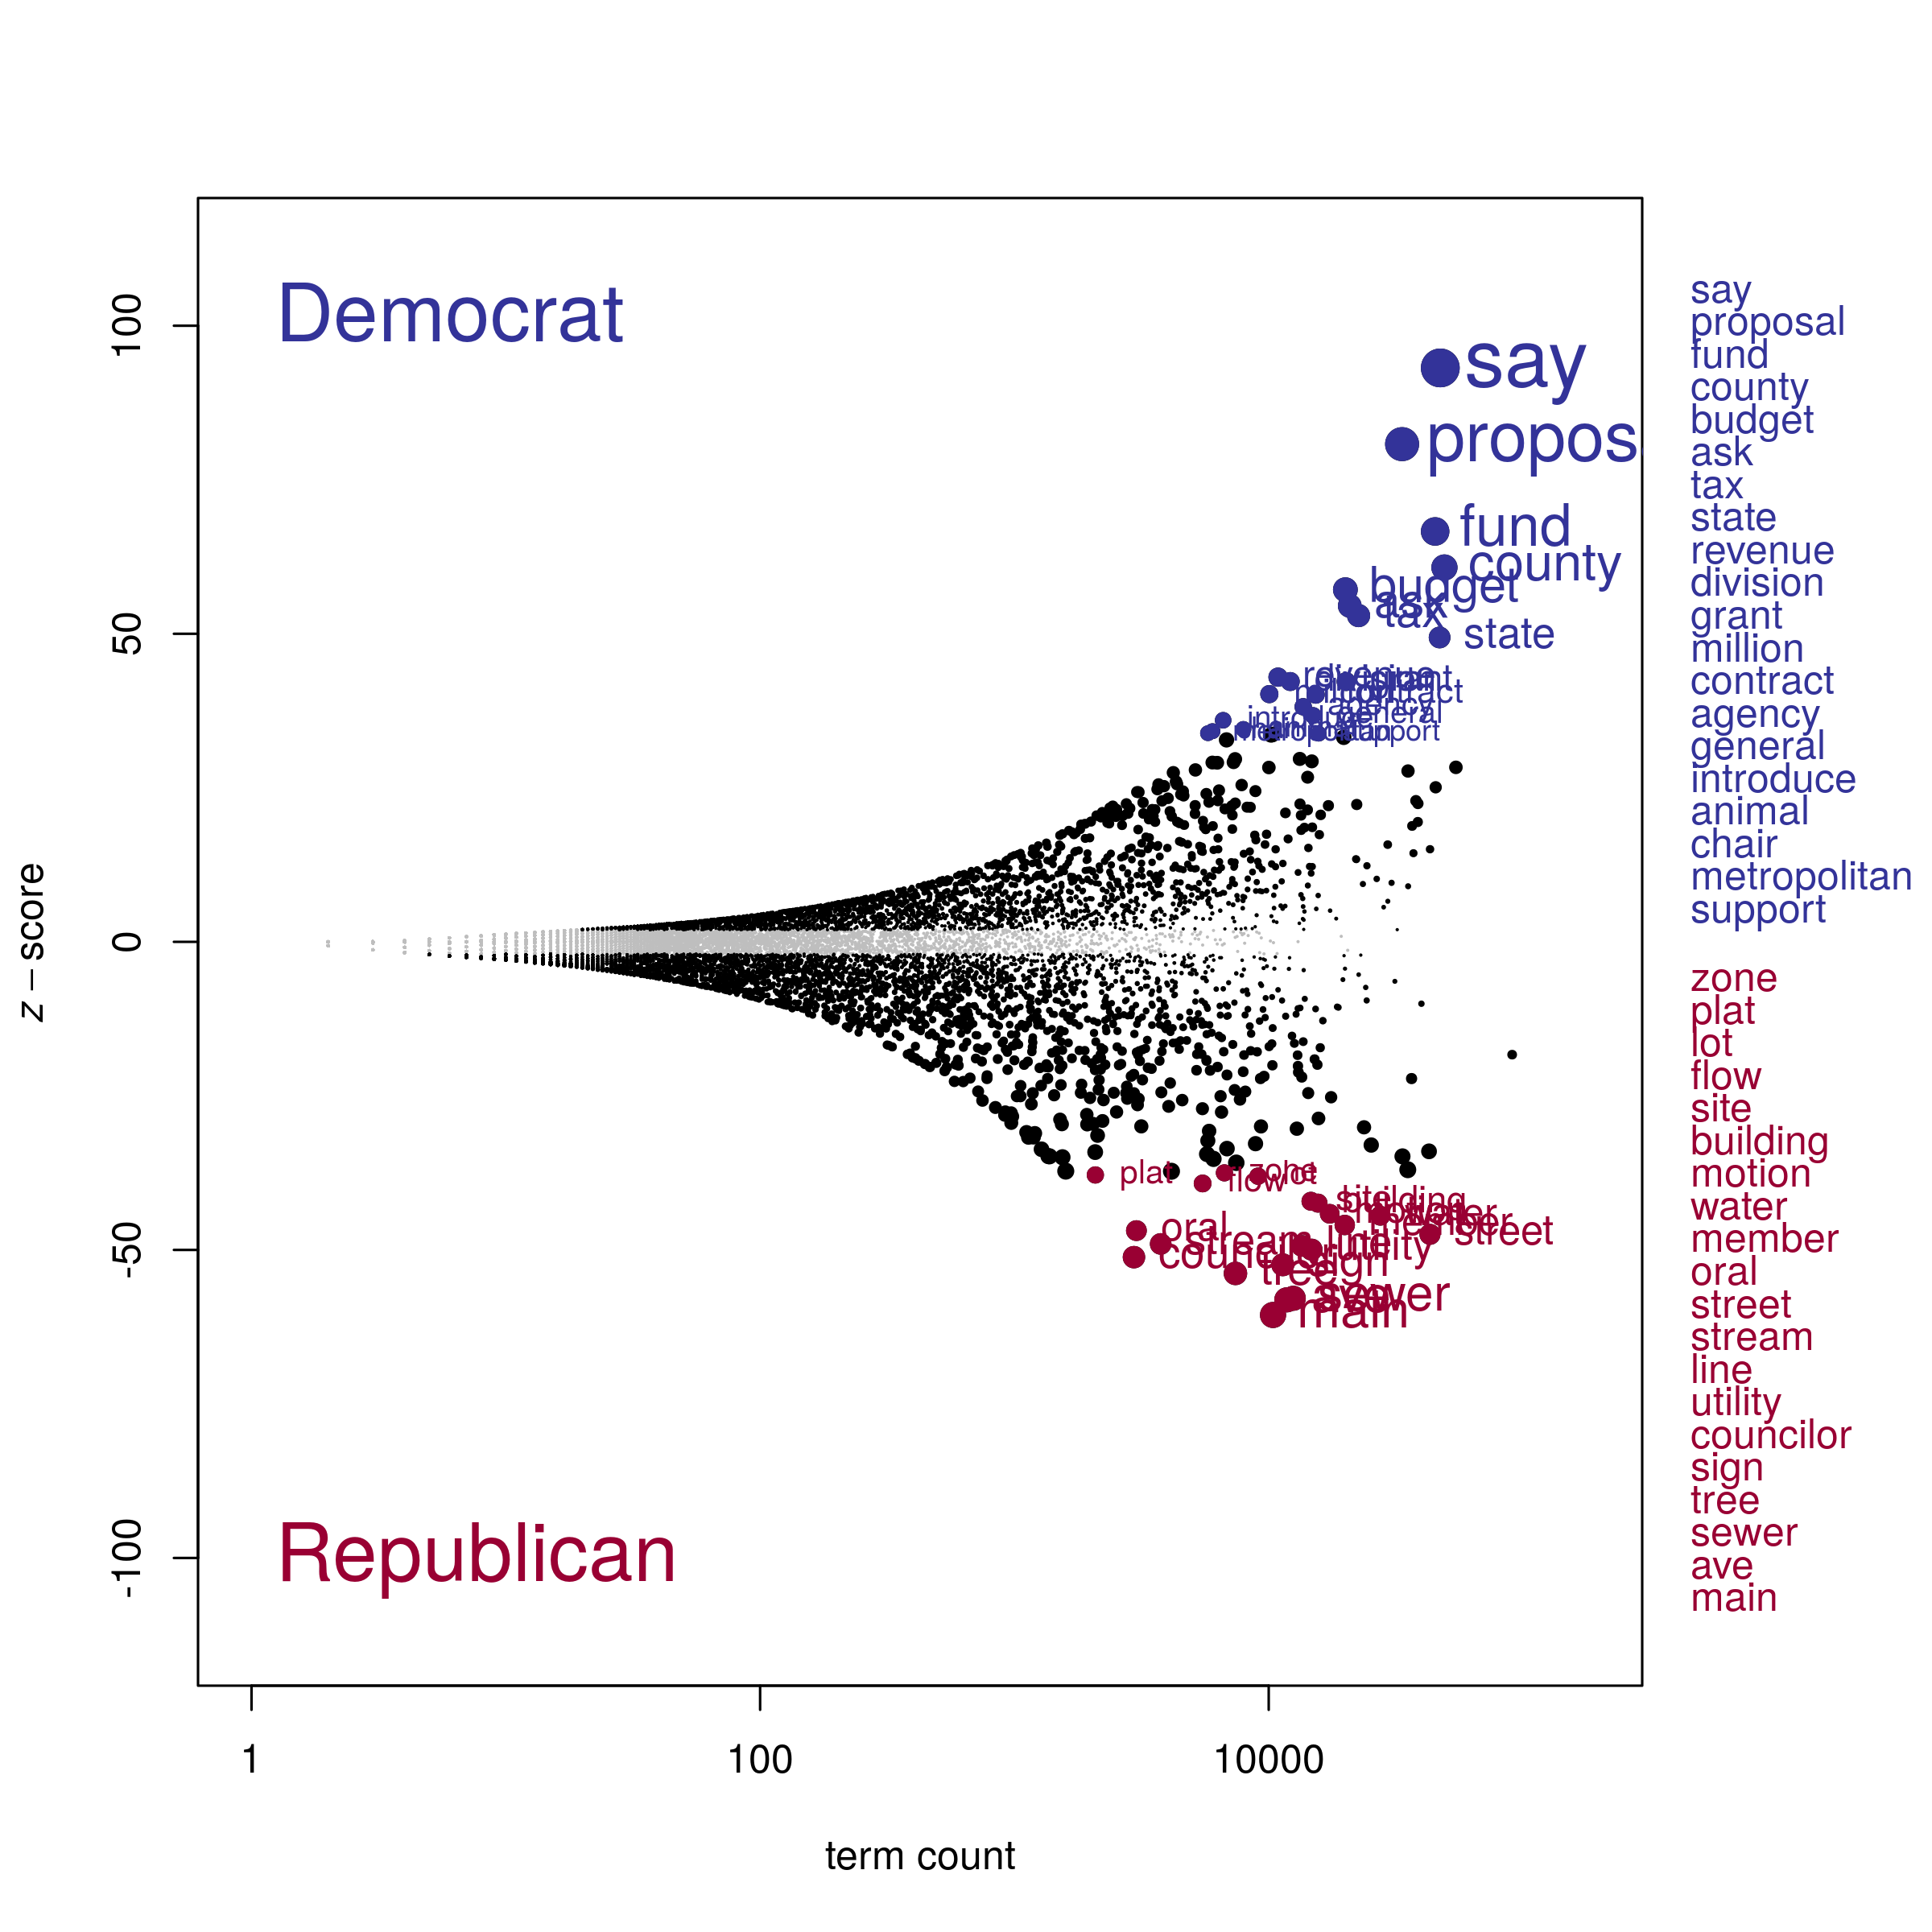
\includegraphics[width=5cm]{../figures/fightinWordsIN.png}}
%	\hfill
%	\subfigure{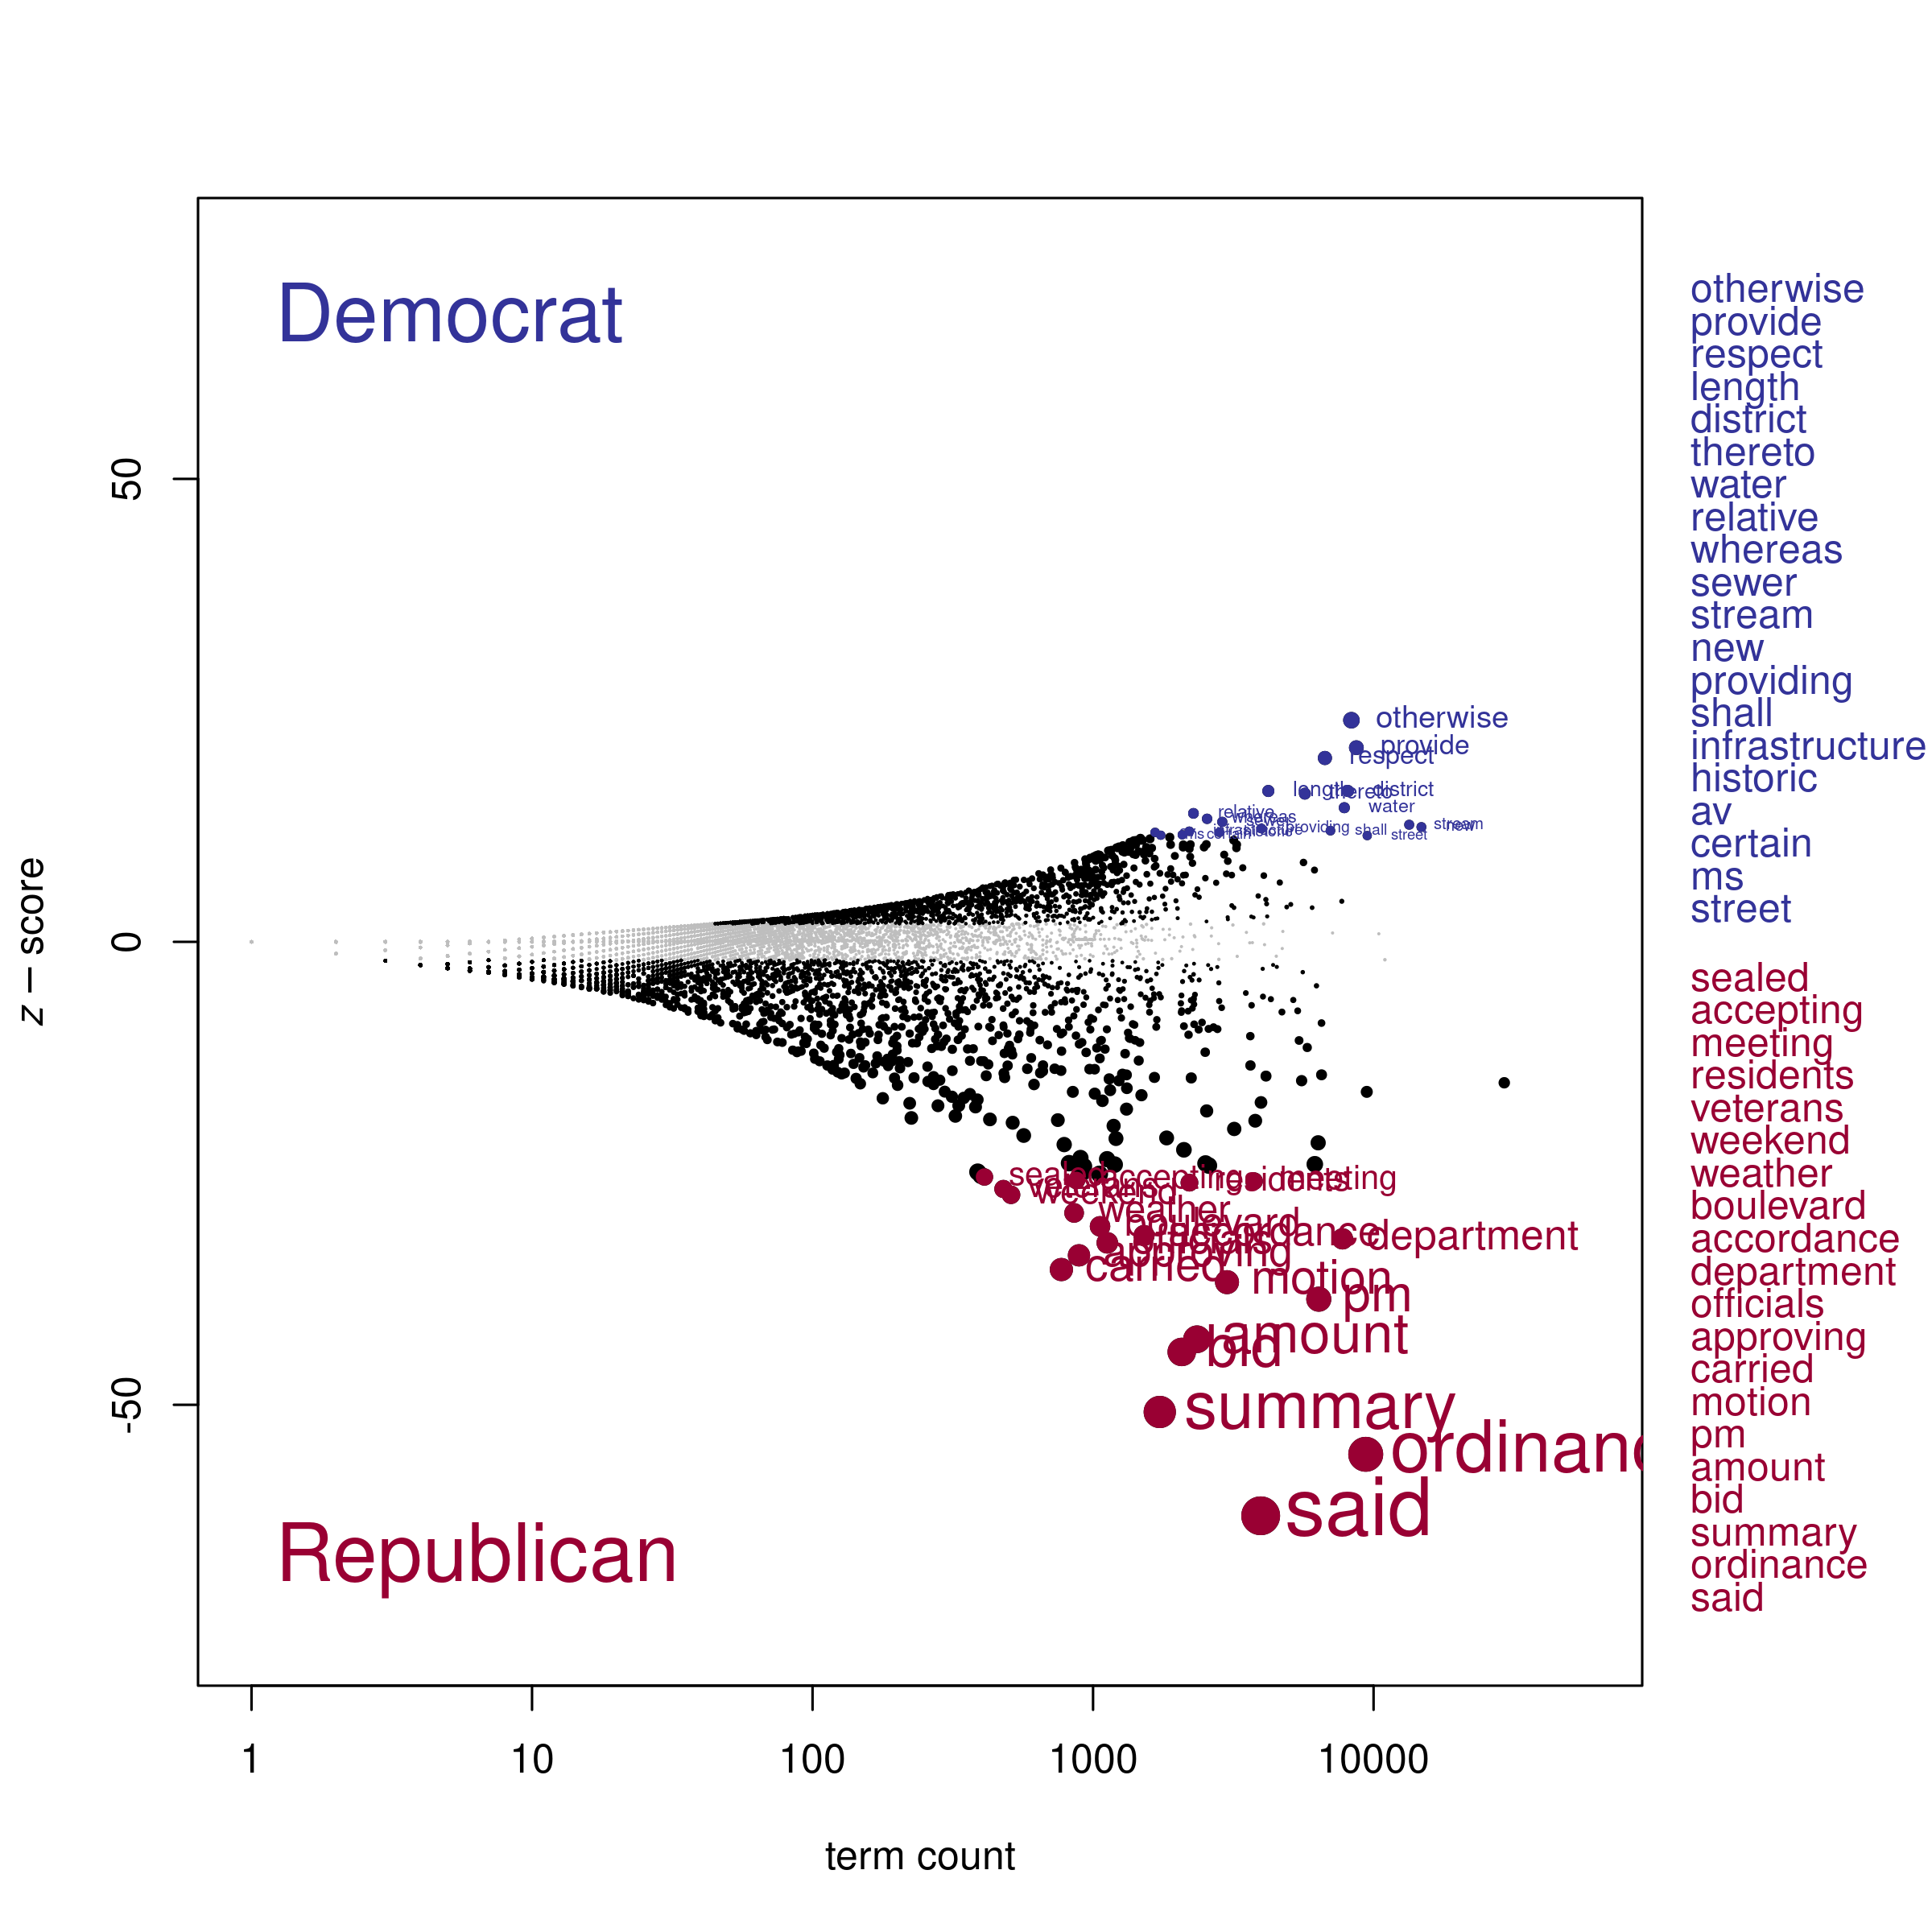
\includegraphics[width=5cm]{../figures/fightinWordsLA.png}}
%\end{figure}
%\end{frame}

\begin{frame}{Fightin' Words - Monroe et al. (2008)}
\linespread{1.5}
\begin{itemize}
	\item Goal: Split words based on one binary variable (party)
	\item Find the most Democratic and most Republican words
	\item Problem: Text mostly consists of meaningless words
	\item Solution: Set prior based on expected distribution of words in random text
	\item Method provides a z-Score indicating the degree to which a word is preferred by one party
	\item Very fast to compute
\end{itemize}
\end{frame}

\begin{frame}{Fightin' Words (Indiana)}
	% latex table generated in R 3.4.1 by xtable 1.8-2 package
% Fri Oct 20 10:49:17 2017
\begin{table}[ht]
\centering
\begingroup\fontsize{9pt}{10pt}\selectfont
\begin{tabular}{lrlr}
  \hline
Word (D) & z-Score (D) & Word (R) & z-Score (R) \\ 
  \hline
said & 86.20 & request & 69.41 \\ 
  proposal & 70.98 & member & 67.45 \\ 
  fund & 59.22 & street & 47.84 \\ 
  county & 54.15 & motion & 46.35 \\ 
  asked & 52.62 & councilor & 45.69 \\ 
  budget & 49.40 & main & 44.34 \\ 
  stated & 46.90 & goods & 44.33 \\ 
  tax & 41.79 & use & 43.43 \\ 
  fort & 41.17 & tree & 42.77 \\ 
  ms & 40.76 & amp & 42.48 \\ 
  division & 38.01 & water & 41.45 \\ 
  million & 36.62 & downtown & 40.66 \\ 
  grants & 35.21 & pm & 39.60 \\ 
  introduced & 34.85 & sign & 39.28 \\ 
  contract & 34.36 & st & 38.23 \\ 
  revenue & 34.33 & plan & 38.20 \\ 
  general & 34.17 & rd & 37.71 \\ 
  chair & 32.01 & site & 37.19 \\ 
  brown & 31.86 & docket & 37.03 \\ 
  federal & 31.46 & trees & 36.56 \\ 
  metropolitan & 31.25 & plat & 36.15 \\ 
  management & 30.69 & old & 35.44 \\ 
  agency & 30.35 & residential & 34.65 \\ 
  approves & 29.66 & area & 34.31 \\ 
  authorizes & 29.11 & variance & 33.50 \\ 
  technology & 28.45 & th & 33.20 \\ 
  provide & 27.43 & utility & 33.11 \\ 
  dollars & 27.30 & ordinance & 32.04 \\ 
  consolidated & 26.29 & carter & 31.40 \\ 
  justice & 25.93 & approve & 31.40 \\ 
  parks & 25.79 & building & 30.78 \\ 
  lewis & 25.73 & feet & 30.16 \\ 
  increase & 25.66 & news & 29.37 \\ 
  digest & 25.60 & city & 29.26 \\ 
  support & 25.43 & lots & 29.19 \\ 
  oliver & 25.43 & lot & 28.89 \\ 
  animal & 25.02 & aid & 28.54 \\ 
  gray & 24.72 & overlay & 28.53 \\ 
  capital & 24.54 & home & 28.52 \\ 
  services & 24.53 & democrat & 28.40 \\ 
  amends & 23.84 & republican & 28.25 \\ 
  criminal & 23.70 & uses & 28.05 \\ 
  enterprise & 23.62 & must & 27.57 \\ 
  mayors & 23.51 & legal & 26.64 \\ 
  court & 22.90 & zoning & 26.53 \\ 
  township & 22.86 & councilors & 26.50 \\ 
  controls & 22.54 & river & 26.48 \\ 
  funded & 22.28 & stellar & 26.40 \\ 
  referred & 22.16 & common & 26.15 \\ 
  fiscal & 22.10 & rep & 26.03 \\ 
   \hline
\end{tabular}
\endgroup
\caption{Top 50 democratic and Republican words (Indiana), according to the informed 
             Dirichlet model of Monroe et al. (2008).} 
\label{tabFightinIN}
\end{table}


%	% latex table generated in R 3.4.1 by xtable 1.8-2 package
% Fri Oct 20 10:49:17 2017
\begin{table}[ht]
\centering
\begingroup\fontsize{9pt}{10pt}\selectfont
\begin{tabular}{lrlr}
  \hline
Word (D) & z-Score (D) & Word (R) & z-Score (R) \\ 
  \hline
said & 86.20 & request & 69.41 \\ 
  proposal & 70.98 & member & 67.45 \\ 
  fund & 59.22 & street & 47.84 \\ 
  county & 54.15 & motion & 46.35 \\ 
  asked & 52.62 & councilor & 45.69 \\ 
  budget & 49.40 & main & 44.34 \\ 
  stated & 46.90 & goods & 44.33 \\ 
  tax & 41.79 & use & 43.43 \\ 
  fort & 41.17 & tree & 42.77 \\ 
  ms & 40.76 & amp & 42.48 \\ 
  division & 38.01 & water & 41.45 \\ 
  million & 36.62 & downtown & 40.66 \\ 
  grants & 35.21 & pm & 39.60 \\ 
  introduced & 34.85 & sign & 39.28 \\ 
  contract & 34.36 & st & 38.23 \\ 
  revenue & 34.33 & plan & 38.20 \\ 
  general & 34.17 & rd & 37.71 \\ 
  chair & 32.01 & site & 37.19 \\ 
  brown & 31.86 & docket & 37.03 \\ 
  federal & 31.46 & trees & 36.56 \\ 
  metropolitan & 31.25 & plat & 36.15 \\ 
  management & 30.69 & old & 35.44 \\ 
  agency & 30.35 & residential & 34.65 \\ 
  approves & 29.66 & area & 34.31 \\ 
  authorizes & 29.11 & variance & 33.50 \\ 
  technology & 28.45 & th & 33.20 \\ 
  provide & 27.43 & utility & 33.11 \\ 
  dollars & 27.30 & ordinance & 32.04 \\ 
  consolidated & 26.29 & carter & 31.40 \\ 
  justice & 25.93 & approve & 31.40 \\ 
  parks & 25.79 & building & 30.78 \\ 
  lewis & 25.73 & feet & 30.16 \\ 
  increase & 25.66 & news & 29.37 \\ 
  digest & 25.60 & city & 29.26 \\ 
  support & 25.43 & lots & 29.19 \\ 
  oliver & 25.43 & lot & 28.89 \\ 
  animal & 25.02 & aid & 28.54 \\ 
  gray & 24.72 & overlay & 28.53 \\ 
  capital & 24.54 & home & 28.52 \\ 
  services & 24.53 & democrat & 28.40 \\ 
  amends & 23.84 & republican & 28.25 \\ 
  criminal & 23.70 & uses & 28.05 \\ 
  enterprise & 23.62 & must & 27.57 \\ 
  mayors & 23.51 & legal & 26.64 \\ 
  court & 22.90 & zoning & 26.53 \\ 
  township & 22.86 & councilors & 26.50 \\ 
  controls & 22.54 & river & 26.48 \\ 
  funded & 22.28 & stellar & 26.40 \\ 
  referred & 22.16 & common & 26.15 \\ 
  fiscal & 22.10 & rep & 26.03 \\ 
   \hline
\end{tabular}
\endgroup
\caption{Top 50 democratic and Republican words (Indiana), according to the informed 
             Dirichlet model of Monroe et al. (2008).} 
\label{tabFightinIN}
\end{table}


\end{frame}

%\begin{frame}{Latent Dirichlet Allocation}
%% latex table generated in R 3.4.1 by xtable 1.8-2 package
% Fri Oct 20 13:14:52 2017
\begin{table}[ht]
\centering
\begingroup\fontsize{9pt}{10pt}\selectfont
\begin{tabular}{lrlr}
  \hline
Word (D) & Instances (D) & Word (R) & Instances (R) \\ 
  \hline
city & 42493 & will & 53761 \\ 
  said & 40480 & city & 36210 \\ 
  county & 39209 & street & 21207 \\ 
  proposal & 29019 & board & 19496 \\ 
  public & 27070 & water & 18637 \\ 
  council & 23492 & plan & 18241 \\ 
  shall & 23162 & public & 14327 \\ 
  department & 22926 & use & 13233 \\ 
  services & 22703 & information & 13062 \\ 
  fund & 21661 & development & 12916 \\ 
  will & 20697 & department & 11554 \\ 
  new & 19000 & area & 11270 \\ 
  stated & 18794 & shall & 11247 \\ 
  project & 18538 & fire & 10861 \\ 
  property & 18378 & can & 10748 \\ 
  budget & 16631 & must & 10633 \\ 
  community & 16236 & park & 10493 \\ 
  asked & 16231 & building & 10356 \\ 
  tax & 14549 & motion & 10168 \\ 
  board & 14363 & ordinance & 9625 \\ 
  state & 13964 & request & 9512 \\ 
  office & 13818 & council & 9098 \\ 
  program & 13536 & community & 9072 \\ 
  year & 13376 & meeting & 8990 \\ 
  service & 13312 & ave & 8555 \\ 
  provide & 13138 & service & 8040 \\ 
  one & 13066 & construction & 7999 \\ 
  section & 12669 & one & 7885 \\ 
  work & 11986 & property & 7741 \\ 
  information & 11886 & also & 7492 \\ 
  development & 11854 & per & 7442 \\ 
  committee & 11802 & required & 7407 \\ 
  district & 11584 & home & 7334 \\ 
  time & 11466 & center & 7316 \\ 
  total & 10965 & made & 7301 \\ 
  general & 10731 & site & 7279 \\ 
  parks & 10704 & business & 7222 \\ 
  system & 10668 & time & 7157 \\ 
  digest & 10481 & services & 7140 \\ 
  police & 10474 & housing & 7111 \\ 
  management & 10433 & new & 7006 \\ 
  park & 10356 & within & 6910 \\ 
  also & 10112 & date & 6818 \\ 
  division & 9964 & year & 6768 \\ 
  street & 9853 & following & 6754 \\ 
  resolution & 9768 & road & 6629 \\ 
  contract & 9763 & member & 6450 \\ 
  ordinance & 9456 & inc & 6367 \\ 
  safety & 9362 & number & 6360 \\ 
  code & 9342 & day & 6254 \\ 
   \hline
\end{tabular}
\endgroup
\caption{Top 50 Democratic and Republican words (Indiana), according to LDA. 
             Topic ownership is determined by the ratio of Democratic to Republican tokens in 
             it (both weighted by the total number of tokens per party). The instances of each 
             token type are then summed across all topics owned by the party.} 
\label{tabLDAIN}
\end{table}


%\end{frame}

\begin{frame}{Structural Topic Model - Roberts et al. (2014)}
\linespread{1.5}
\begin{itemize}
	\item Topic models find clusters of semantically related words in texts --> i.e. topics
	\item As a clustering method, LDA doesn't explicitly allow for covariates (although post-hoc comparison is possible)
	\item The structural topic model extends this approach to explicitly include (multiple) covariates
	\item Our covariates: Party + City Population
\end{itemize}
\end{frame}

\begin{frame}{Structural Topic Model (Indiana)}
% latex table generated in R 3.4.3 by xtable 1.8-2 package
% Tue Dec 26 20:59:22 2017
\begin{table}[ht]
\centering
\scriptsize
\begin{tabular}{llllll}
  \hline
-0.027 & -0.022 & -0.016 & -0.011 & -0.011 & -0.01 \\ 
  \hline
city & school & downtown & city & \cellcolor{blue!25}trash & \cellcolor{blue!25}housing \\ 
  ordinance & community & business & department & city & property \\ 
  approve & program & project & mayor & \cellcolor{blue!25}waste & program \\ 
  resolution & student & city & police & day & \cellcolor{blue!25}fund \\ 
  property & \cellcolor{blue!25}education & \cellcolor{blue!25}development & officer & \cellcolor{blue!25}recycle & home \\ 
  purchase & \cellcolor{blue!25}university & new & public & street & city \\ 
  area & national & center & citizen & collection & project \\ 
  department & award & \cellcolor{blue!25}economic & work & resident & neighborhood \\ 
  contract & high & company & safety & \cellcolor{blue!25}recycling & \cellcolor{blue!25}grant \\ 
  service & year & community & resident & snow & unit \\ 
   \hline
\end{tabular}
\caption{Top Democratic topics and words}%\caption{Top Democratic topics and words (Indiana), according to STM. 
%The words are the top words for the most Democratic/Republican topic, determined
%by the size (and significance) of the coefficient (see table header) of the party covariate.} 
\label{tabSTMINDem}
\end{table}

 %../tables/stmTopWordsINDem.tex
\end{frame}

\begin{frame}{Structural Topic Model (Indiana)}
% latex table generated in R 3.4.2 by xtable 1.8-2 package
% Mon Nov 13 15:36:58 2017
\begin{table}[ht]
\centering
\begin{tabular}{llllll}
  \hline
0.024 & 0.019 & 0.019 & 0.016 & 0.016 & 0.016 \\ 
  \hline
motion & plan & inc & request & council & \cellcolor{red!25} traffic \\ 
  second & \cellcolor{red!25} zone & electr & board & citi & amp \\ 
  made & applic & build & member & ordin & vehicl \\ 
  approv & \cellcolor{red!25} properti & construct & servic & common & stop \\ 
  mayor & approv & home & \cellcolor{red!25} street & councilor & sign \\ 
  present & sign & street & approv & amend & \cellcolor{red!25} road \\ 
  state & \cellcolor{red!25} site & meridian & purchas & resolut & block \\ 
  will & locat & servic & citi & adopt & signal \\ 
  citi & commiss & west & move & wherea & \cellcolor{red!25} street \\ 
  council & file & main & good & approv & driver \\ 
   \hline
\end{tabular}
%\caption{Top Republican topics and words (Indiana), according to STM. 
%The words are the top words for the most Democratic/Republican topic, determined
%by the size (and significance) of the coefficient (see table header) of the party covariate.} 
\label{tabSTMINRep}
\end{table}

 %../tables/stmTopWordsINRep.tex
\end{frame}

\section{Conclusion}
\begin{frame}{Conclusion}
\linespread{1.5}
\large
\begin{itemize}
	%\item Hierarchical clustering only creates 'topics' if content is VERY similar
	%\item Fightin words is extremely effective at forcing the text into two categories, but also somewhat limited
	%\item LDA is sensitive to preprocessing, but the most flexible
	%\item STM works too, but also very sensitive to duplicate content
	\item Manual vs. automatic analysis of government websites
	\item Our pipeline facilities scalable comparative analysis
	
	\vspace{5mm}
	\item Partisanship affects website content:
	\item Democrats focus on raising and spending money
	\item Republicans focus on infrastructure and utilities
\end{itemize}
\end{frame}

\end{document}